\documentclass{article}

\usepackage{graphicx}
\usepackage{tikz}
\usepackage{tikzsymbols}
\usetikzlibrary{calc,patterns,shapes.geometric}
\pagestyle{empty}
\usepackage[margin=0pt]{geometry}
\geometry{papersize={14in,12in}}

\def\centerarc[#1](#2)(#3:#4:#5){\draw[#1] ($(#2)+({#5*cos(#3)},{#5*sin(#3)})$) arc (#3:#4:#5);}

\begin{document}
	\begin{figure}
		\centering
		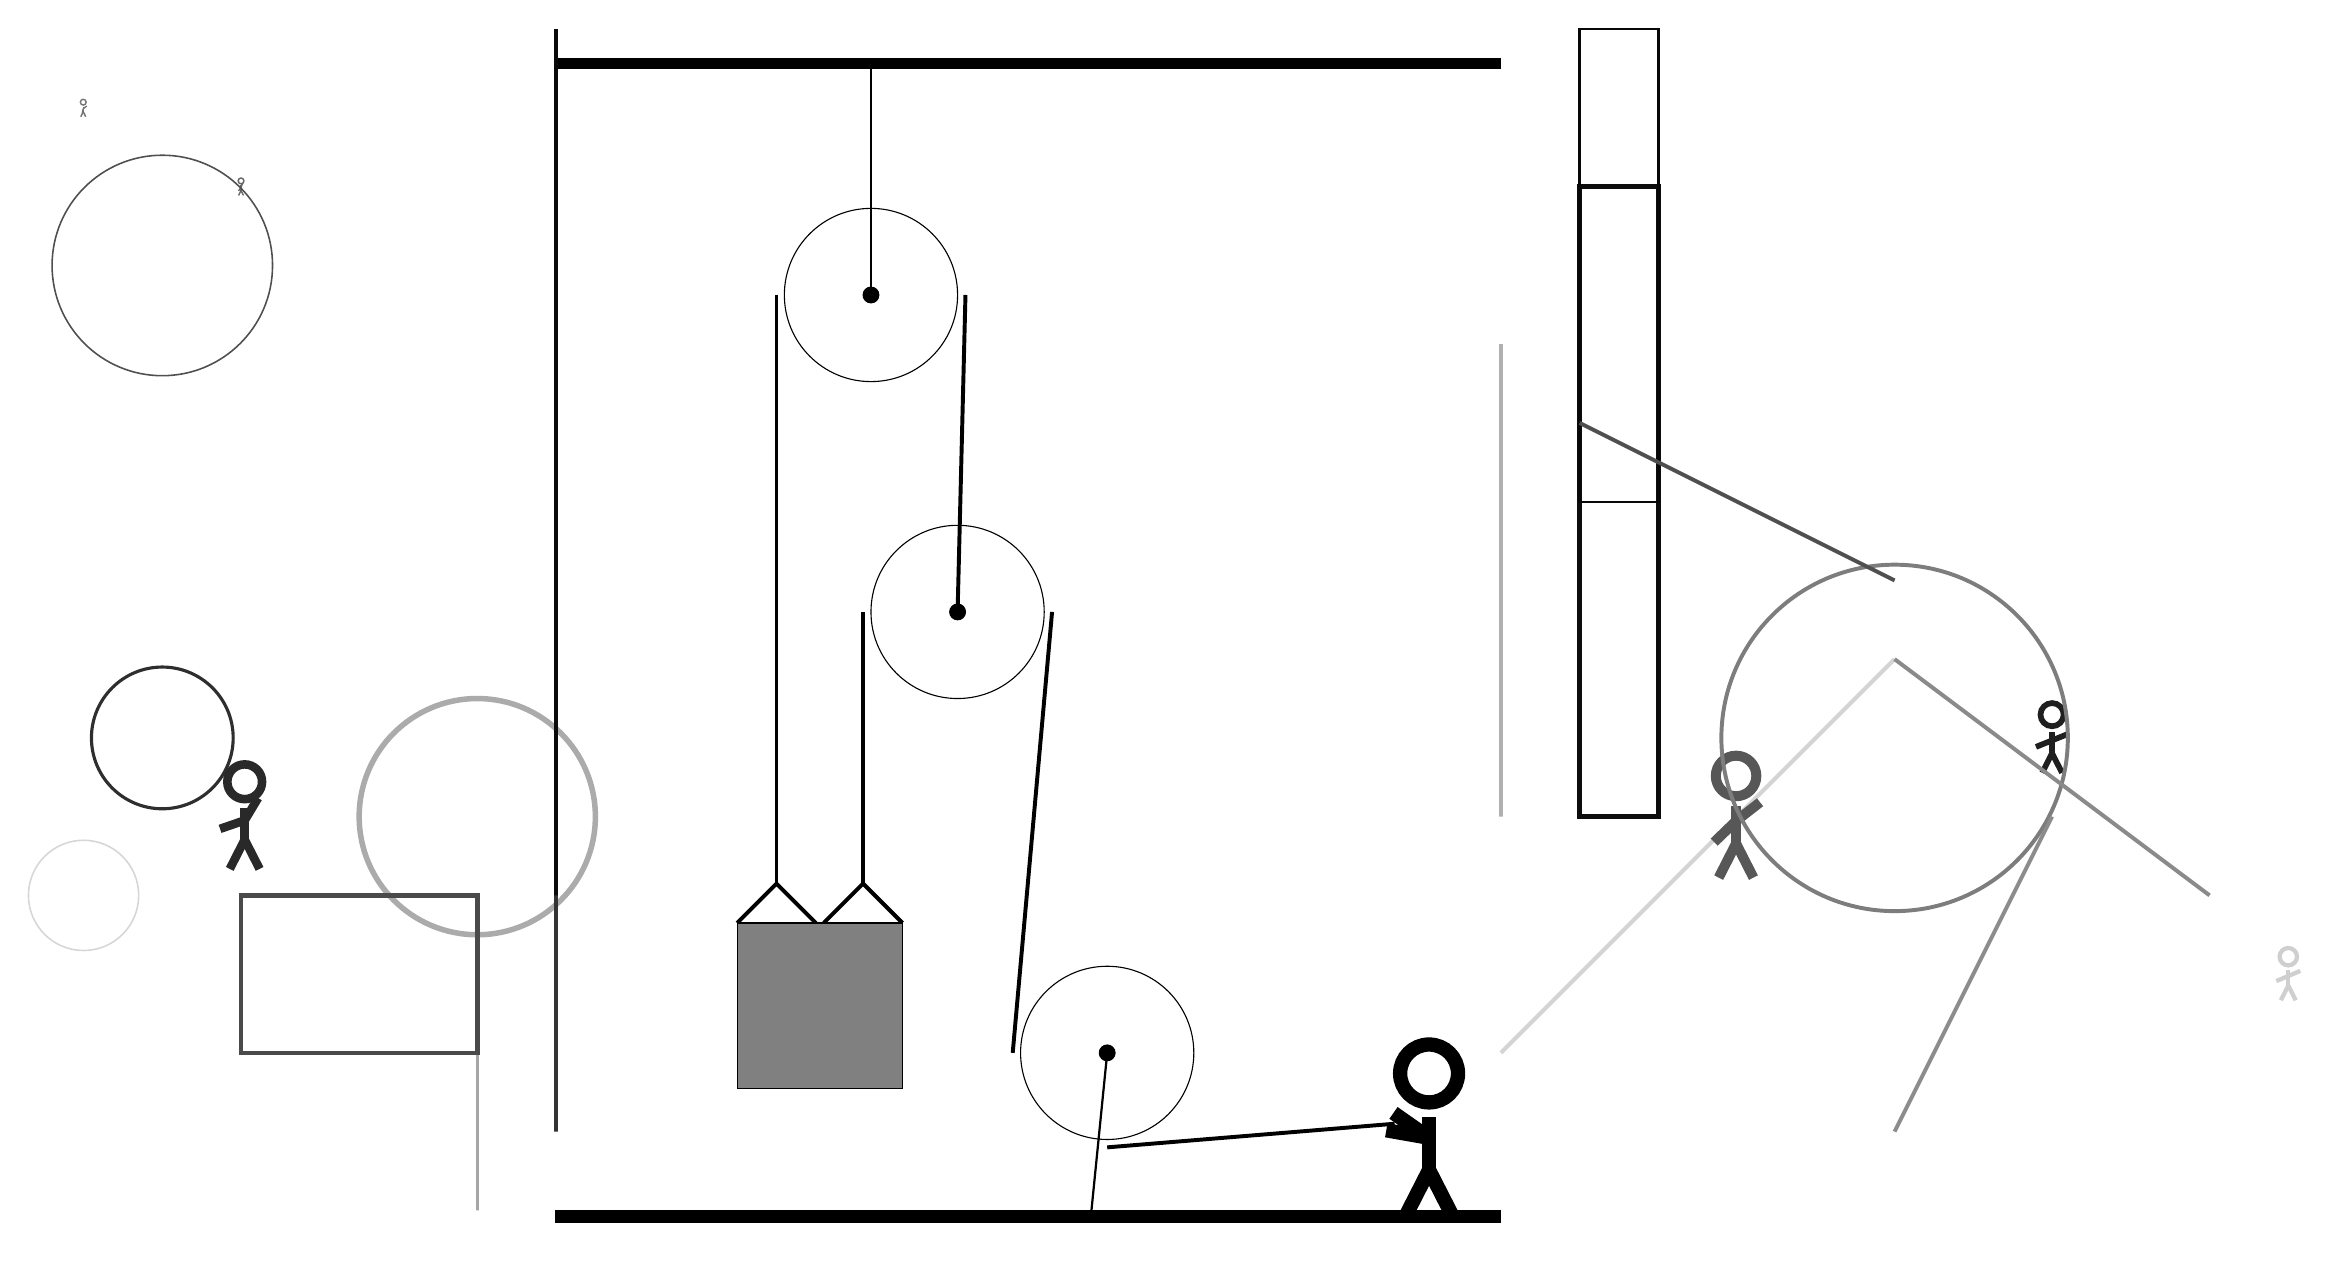
\begin{tikzpicture}
			%%%%% START %%%%%
			
			\draw[fill=black] (-2, 11.5) rectangle (10, 11.625);
			
			\draw[line width=0.5mm, color=black!17](15, 4) -- (10, -1);
			
			\node[line width=0.7mm, color=black!66] at (13, 2) {\Strichmaxerl[7][44][38]};
			\node[line width=0.3mm, color=black!88] at (17, 3) {\Strichmaxerl[4][22][22]};
			\draw [line width=0.5mm, color=black!51](15, 3) circle (2.2);
			\draw[line width=0.5mm, color=black!31] (10, 2) rectangle (10, 8);
			\draw[line width=0.6mm, color=black!95] (12, 10) rectangle (11, 2);
			
			\draw [line width=0.4mm, color=black!82](-7, 3) circle (0.9);
			\draw [line width=0.7mm, color=black!33](-3, 2) circle (1.5);
			\draw[line width=0.4mm, color=black!96] (-2, 0) rectangle (-2, 12);
			\node[line width=0.5mm, color=black!54] at (-8, 11) {\Strichmaxerl[1][78][36]};
			\node[line width=0.6mm, color=black!19] at (20, 0) {\Strichmaxerl[3][23][23]};
			
			\node[line width=0.7mm, color=black!84] at (-6, 2) {\Strichmaxerl[6][19][59]};
			\node[line width=0.2mm, color=black!60] at (-6, 10) {\Strichmaxerl[1][54][70]};
			\draw[line width=0.4mm, color=black!35] (-3, -3) rectangle (-3, 1);
			\draw[line width=0.3mm, color=black!97] (12, 6) rectangle (11, 12);
			\draw [line width=0.2mm, color=black!16](-8, 1) circle (0.7);
			
			\draw[line width=0.5mm, color=black!46](15, 4) -- (19, 1);
			\draw[line width=0.5mm, color=black!80] (-2, -2) rectangle (-2, 1);
			\draw[line width=0.5mm, color=black!45](15, -2) -- (17, 2);
			
			\draw[line width=0.6mm, color=black!71] (-3, -1) rectangle (-6, 1);
			\draw[line width=0.5mm, color=black!69](11, 7) -- (15, 5);
			
			\draw [line width=0.2mm, color=black!69](-7, 9) circle (1.4);
			
			\draw (2, 8.625) circle (1.1);
			\draw[fill=black] (2, 8.625) circle (0.1);
			\draw[thick] (2, 8.625) -- (2, 11.5);
			
			\draw (3.1, 4.6) circle (1.1);
			\draw[fill=black] (3.1, 4.6) circle (0.1);
			
			\draw (5, -1) circle (1.1);
			\draw[fill=black] (5, -1) circle (0.1);
			\draw[thick] (5, -1) -- (4.8, -3);
			
			\draw[line width = 0.5mm]  (0.3, 0.65) -- (0.8, 1.15) -- (1.3, 0.65);
			\draw[line width = 0.5mm]  (1.4, 0.65) -- (1.9, 1.15) -- (2.4, 0.65);
			\draw[fill=black!50] (0.3, 0.65) rectangle (2.4, -1.45);
			
			\draw[line width = 0.5mm] (0.8, 8.625) -- (0.8, 1.15);
			\centerarc[line width = 0.5mm](2, 8.625)(0:180:1.2000000000000002);
			\draw[line width = 0.5mm] (3.2, 8.625) -- (3.1, 4.6);
			\draw[line width = 0.5mm] (1.9, 4.6) -- (1.9, 1.15);
			\centerarc[line width = 0.5mm](3.1, 4.6)(0:180:1.2000000000000002);
			\draw[line width = 0.5mm] (4.3, 4.6) -- (3.8, -1);
			\centerarc[line width = 0.5mm](5, -1)(180:270:1.2000000000000002);
			\draw[line width = 0.5mm] (5, -2.2) -- (8.65, -1.9);
			
			\node at (9, -2) {\Strichmaxerl[10][-35][170]};
			
			\draw[fill=black] (-2, -3) rectangle (10, -3.15);
			
			%%%%% END %%%%%
		\end{tikzpicture}
	\end{figure}	
\end{document}